\documentclass[14pt, a4paper]{extarticle}
\usepackage{GOST}
\usepackage{array}
\usepackage{verbatim}
\usepackage[detect-all]{siunitx}
\usepackage{amsmath}
\usepackage{amssymb}
\usepackage[utf8]{inputenc}
\usepackage{hyperref}
\usepackage{tempora}

\makeatletter
\renewcommand\@biblabel[1]{#1.}
\makeatother

\usepackage{listings}
\lstset{ 
	language=python,
	basicstyle=\small\sffamily, 
	numbers=left, 
	numberstyle=\tiny,
	stepnumber=1,
	numbersep=5pt,
	showspaces=false,            
	showstringspaces=false,      
	showtabs=false,             
	frame=single,            % рисовать рамку вокруг кода
	tabsize=4,      
	commentstyle=\color{green},
	keywordstyle=\color{blue}\textbf,
	numberstyle=\scriptsize\color{gray}, % the style that is used for the line-numbers
	rulecolor=\color{black},
	captionpos=t,
	breaklines=true,         % автоматически переносить строки 
	breakatwhitespace=false, % переносить строки по пробелу
	escapeinside={\#*}{*)} 
}

\begin{document}
	
\begin{table}[ht]
	\centering
	\begin{tabular}{|c|p{400pt}|} 
		\hline
		\begin{tabular}[c]{@{}c@{}} 
\includegraphics[scale=1]{baum.jpg} \\\end{tabular} &
		\footnotesize\begin{tabular}[c]{@{}c@{}}\textbf{Министерство~науки~и~высшего~образования~Российской~Федерации}\\\textbf{Федеральное~государственное~бюджетное~образовательное~учреждение}\\\textbf{~высшего~образования}\\\textbf{«Московский~государственный~технический~университет}\\\textbf{имени~Н.Э.~Баумана}\\\textbf{(национальный~исследовательский~университет)»}\\\textbf{(МГТУ~им.~Н.Э.~Баумана)}\\\end{tabular}  \\
		\hline
	\end{tabular}
\end{table}
\noindent\rule{\textwidth}{4pt}
\noindent\rule[14pt]{\textwidth}{1pt}
\hfill 
\noindent
\makebox{ФАКУЛЬТЕТ~}%
\makebox[\textwidth][l]{\underline{~«Информатика и системы управления»~~~~~~~~~~~~~~~~~~~~~~~~~~~~~~~~~}}%
\\
\noindent
\makebox{КАФЕДРА~}%
\makebox[\textwidth][l]{\underline{~«Программное обеспечение ЭВМ и информационные технологии»~}}%


\begin{center}
	\vspace{1.5cm}
	{\bf\huge Отчёт\par}
	{\bf\Large по лабораторной работе № 3\par}
	\vspace{0.7cm}
\end{center}

\noindent
\makebox{\large{\bf Название:}~~~}
\makebox[\textwidth][l]{\large\underline{~ Программно-алгоритмическая реализация моделей~}}\\
\makebox[\textwidth][l]{\large\underline{~на основе ОДУ второго 
		порядка с краевыми условиями II и III рода~}}\\


\noindent
\makebox{\large{\bf Дисциплина:}~~~}
\makebox[\textwidth][l]{\large\underline{~Моделирование~}}\\

\vspace{1.5cm}
\noindent
\begin{tabular}{l c c c c c}
	Студент      & ~ИУ7-65Б~               & \hspace{2.5cm} & \hspace{2cm}                 & &  Д.В. Сусликов \\\cline{2-2}\cline{4-4} \cline{6-6} 
	\hspace{3cm} & {\footnotesize(Группа)} &                & {\footnotesize(Подпись, дата)} & & {\footnotesize(И.О. Фамилия)}
\end{tabular}

\noindent
\begin{tabular}{l c c c c}
	Преподователь & \hspace{5cm}   & \hspace{2cm}                 & & ~~~~~~~В.М. Градов~~~~~~~\\\cline{3-3} \cline{5-5} 
	\hspace{3cm}  &                & {\footnotesize(Подпись, дата)} & & {\footnotesize(И.О. Фамилия)}
\end{tabular}

\vspace{0.6cm}
\begin{center}	
	\vfill
	\large \textit {Москва, 2021}
\end{center}

\thispagestyle {empty}
\pagebreak

% ВВЕДЕНИЕ
\clearpage
\section*{Цель работы:} Получение навыков разработки алгоритмов решения краевой задачи при реализации моделей, построенных на ОДУ второго порядка.
\section*{Исходные данные.} 
1. Задана математическая модель. Квазилинейное уравнение для функции T(x):
\begin{equation*}
	\frac{d}{dx} (\lambda(x)\frac{dT}{dx}) - 4k(T)n^{2}_{p}\sigma(T^4 -T^{4}_{0}) = 0
\end{equation*}
Краевые условия:
\begin{equation*}
	\begin{cases}
		x = 0, -\lambda(T(0))\frac{dT}{dx} = F_0\\
		x = l, -\lambda(T(0))\frac{dT}{dx} = \alpha(T(l) - T_0)
	\end{cases}
\end{equation*}

2. Функции $\lambda(T), k(T)$ заданы в таблице:
\begin{table}[h!]
	\begin{tabular}{|l|l|l|l|l|}
		\hline
		T, K & $\lambda$, ВТ/(см К)        &  & T, K & k, см\textasciicircum{}-1  \\ \hline
		300  & 1.36*10\textasciicircum{}-2 &  & 293  & 2.0*10\textasciicircum{}-2 \\ \hline
		500  & 1.63*10\textasciicircum{}-2 &  & 1278 & 5.0*10\textasciicircum{}-2 \\ \hline
		800  & 1.81*10\textasciicircum{}-2 &  & 1528 & 7.8*10\textasciicircum{}-2 \\ \hline
		1100 & 1.98*10\textasciicircum{}-2 &  & 1677 & 1.0*10\textasciicircum{}-1 \\ \hline
		2000 & 2.50*10\textasciicircum{}-2 &  & 2000 & 1.3*10\textasciicircum{}-1 \\ \hline
		2400 & 2.74*10\textasciicircum{}-2 &  & 2400 & 2.0*10\textasciicircum{}-1 \\ \hline
	\end{tabular}
\end{table}\par
3. Разностная схема с разностным краевым условием при x = 0\\
$A_ny_{n-1} - B_ny_n + C_ny_{n+1} = -D_n, 1 <= n <= N - 1$\\
$A_n = \frac{\chi_{n-\frac{1}{2}}}{h}$\\
$C_n = \frac{\chi_{n+\frac{1}{2}}}{h}$\\
$B_n = A_n + C_n$\\
$D_n = f_nh$\\
Система с краевыми условиями решается методом прогонки\\
Для величин численно вычисляя $\chi_{n+-\frac{1}{2}}$ можно получить различные приближенные выражения, интеграл методом трапеций или методом средних. Для вычислений будет использоваться метод средних: \\
$\chi_{n+-\frac{1}{2}}$ = $\frac{k_n + k_{+-1}}{2}$\\
Разностный аналог краевого условия при х=0: \\
$\chi_{\frac{1}{2}}y_0 - \chi_{\frac{1}{2}}y_1 = hF_0 + \frac{h^2}{4}(f_{\frac{1}{2}} + f_0)$\\
Простая аппроксимация:\\
$f_{\frac{1}{2}} = \frac{f_0 + f_1}{2}$\\
Также:\\
$F_N = \alpha_n(y_N - T_0)$ и \\
$F_{N- \frac{1}{2}} = \chi_{N-\frac{1}{2}}\frac{y_{N-1} - y_N}{h}$\par
4. Значения параметров:
$n_p=1.4$\\
$l = 0.2$ см\\
$T_0 = 300$ K\\
$\sigma=5.688*10^-12$ Вт/см$^2$К$^4$\\
$F_0 = 100$ Вт/см$^2$\\
$\alpha = 0.05$ Вт/(см$^2$*К)\par
5. Выход из итераций по температуре и балансу:
\begin{equation*}
	max|\frac{y_n^s-y_n^{s-1}}{den}| \leq\epsilon_1, n = 0..N
\end{equation*}
и
\begin{equation*}
	max|\frac{f_1^s - f_2^s}{f_1^s}| \leq\epsilon_2
\end{equation*}
где
\begin{equation*}
	f_1 = F_0 - \alpha(T(l) - T_0) \text{и} f_2 4n_p^2\sigma\int_{0}^{l}k(x)(T^4 - T_0^4)
\end{equation*}
\textbf{Физическое содержание задачи} (для понимания получаемых результатов при отладке программы).\\
Сформулированная математическая модель описывает температурное поле T(x) в плоском слое с внутренними стоками тепловой энергии. Можно представить, что это стенка из полупрозрачного материала, например, кварца или сапфира, нагружаемая тепловым потоком на одной из поверхностей (у нас - слева). Другая поверхность (справа) охлаждается потоком воздуха, температура которого равна T0. Например, данной схеме удовлетворяет цилиндрическая оболочка, ограничивающая разряд в газе, т.к. при больших диаметрах цилиндра стенку можно считать плоской. При высоких температурах раскаленный слой начинает объемно излучать, что описывает второе слагаемое в (1) (закон Кирхгофа). Зависимость от температуры излучательной способности материала очень резкая. При низких температурах стенка излучает очень слабо, второе слагаемое в уравнении (1) практически отсутствует. Функции $\lambda(T), k(T)$ являются, соответственно, коэффициентами теплопроводности и оптического поглощения материала стенки.

\section*{Результаты}
1. Представить разностный аналог краевого условия при x=l и его краткий вывод интегро-интерполяционным методом.	\\
Пусть $F = -\lambda(T)\frac{dT}{dx}$\\
Тогда\\
$\frac{dF}{dx} + f(T) = 0$, где $f(T) = - 4k(T)n^{2}_{p}\sigma(T^4 -T^{4}_{0})$\\
Проинтегрируем на отрезке $[x_{N-\frac{1}{2}}, x_N]$, тогда\\
\begin{equation*}
	-\int_{x_{N-\frac{1}{2}}}^{x_n}\frac{dF}{dx}dx+\int_{x_{N-\frac{1}{2}}}^{x_n}f(x)dx = 0 
\end{equation*}
Применим метод трапеций и получим:
\begin{equation*}
	-(F_N - F_{N-\frac{1}{2}})+\frac{h}{4}(f_N+f_{N-\frac{1}{2}}) = 0
\end{equation*}
Используя $F_N = \alpha_n(y_N - T_0)$ и 
$F_{N- \frac{1}{2}} = \chi_{N-\frac{1}{2}}\frac{y_{N-1} - y_N}{h}$
получим:\\
\begin{equation*}
	-(\alpha(y_N-T_0) - \chi_{N-\frac{1}{2}}\frac{y_{N-1} - y_N}{h}) + \frac{h}{4}(f_N + f_{N-\frac{1}{2}}) = 0
\end{equation*}
\begin{equation*}
	-h\alpha(y_N-T_0) + \chi_{N-\frac{1}{2}}(y_{N-1} - y_N)+\frac{h^2}{4}(f_N+f_{N-\frac{1}{2}}) = 0
\end{equation*}
\begin{equation*}
	-\chi_{N-\frac{1}{2}}y_{N-1} + (h\alpha + \chi_{N - \frac{1}{2}})y_N = \frac{h^2}{4}(f_N+f_{N-\frac{1}{2}}) + h\alpha T_0
\end{equation*}

\par
2.График зависимости температуры T(x) от координаты x при заданных выше параметрах.\\
Выяснить, как сильно зависят результаты расчета T(x) и необходимое для этого количество итераций от начального распределения температуры и шага сетки
\begin{figure}[h!]	
	\center{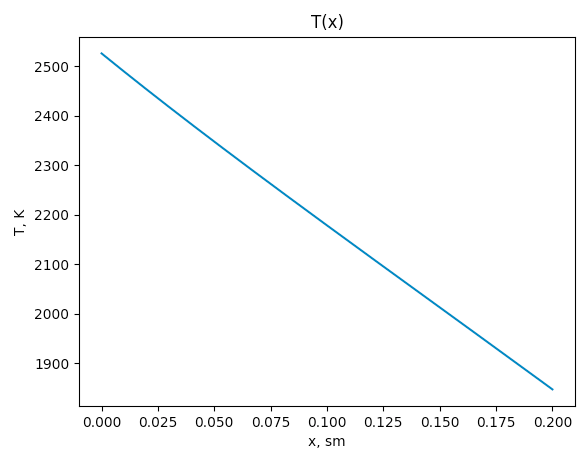
\includegraphics[scale=0.85]{graphics/2.png}}	
\end{figure}\par

\newpage
3. График зависимости T(x) при $F_0=-10$ Вт/см2. \\
Справка. При отрицательном тепловом потоке слева идет съем тепла, поэтому производная $T'(x)$ должна быть положительной.
\begin{figure}[h!]	
	\center{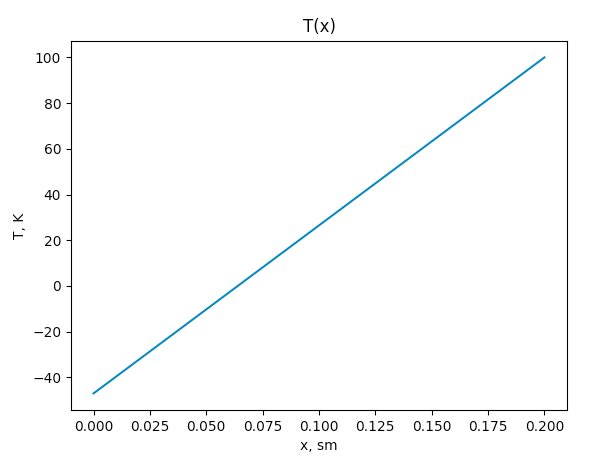
\includegraphics[scale=0.85]{graphics/3.png}}	
\end{figure}\par

\newpage
4. График зависимости T(x) при увеличенных значениях $\alpha(x)$ (например, в 3 раза). Сравнить с п.2.\\
Справка. При увеличении теплосъема и неизменном потоке $F_0$ уровень температур T(x) должен снижаться, а градиент  увеличиваться.
\begin{figure}[h!]	
	\center{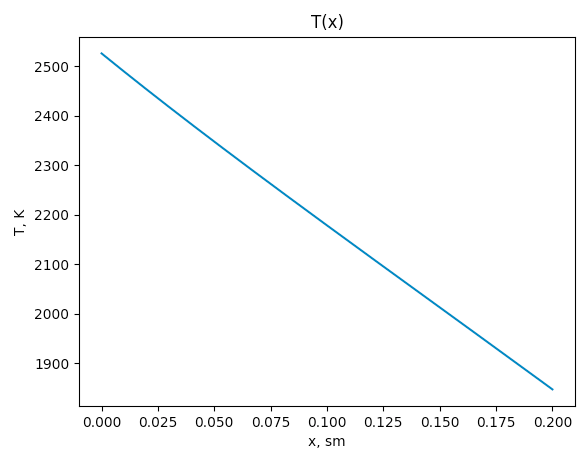
\includegraphics[scale=0.85]{graphics/2.png} \\ $\text{График при } \alpha = 0.05$}	
\end{figure}\par
\newpage
\begin{figure}[h!]	
	\center{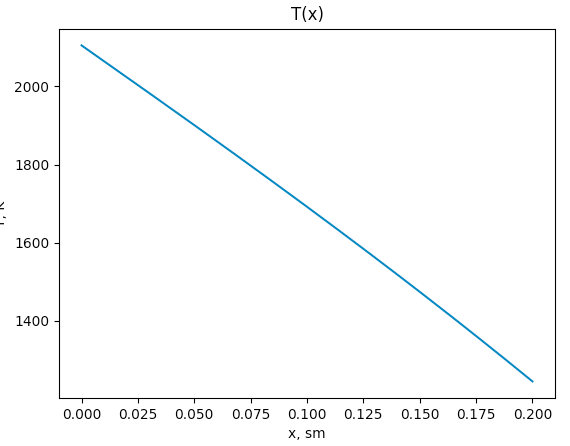
\includegraphics[scale=0.85]{graphics/42.png} \\ $\text{График при } \alpha = 0.1$}	
\end{figure}\par

\begin{figure}[h!]	
	\center{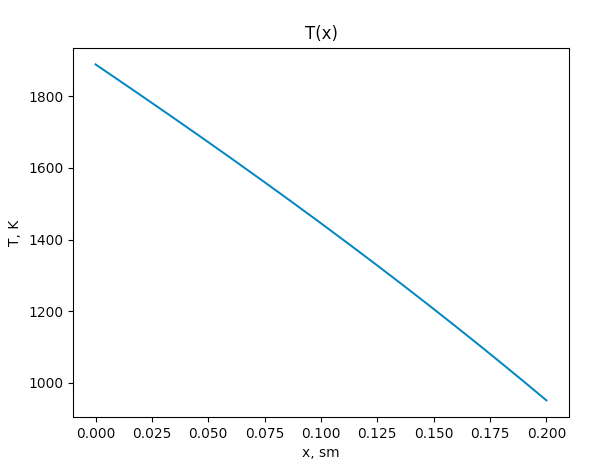
\includegraphics[scale=0.85]{graphics/43.png} \\ $\text{График при } \alpha = 0.15$}	
\end{figure}\par

\newpage
5. График зависимости T(x) при $F_0=0$.\\
Справка. В данных условиях тепловое нагружение отсутствует, причин для нагрева нет, температура стержня должна быть равна температуре окружающей среды $T_0$ (разумеется с некоторой погрешностью, определяемой приближенным характером вычислений).  

\begin{figure}[h!]	
	\center{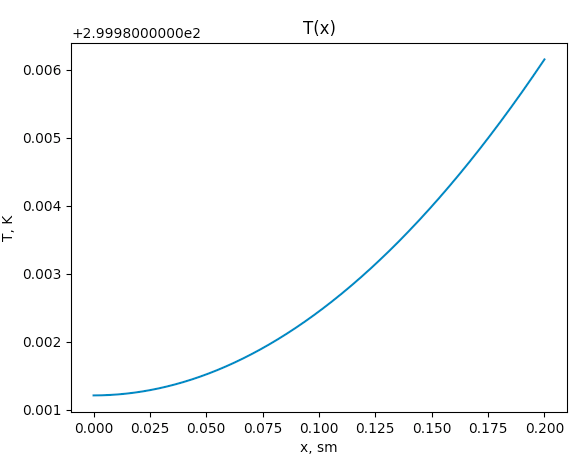
\includegraphics[scale=0.85]{graphics/5.png}}	
\end{figure}\par

\newpage
6. Для указанного в задании исходного набора параметров привести данные по балансу энергии, т.е. значения величин
\begin{equation*}
	f_1 = F_0 - \alpha(T(l) - T_0) \text{и} f_2 4n_p^2\sigma\int_{0}^{l}k(x)(T^4 - T_0^4)
\end{equation*}
Каковы использованные в работе значения точности выхода из итераций $\epsilon_1$(по темпера-туре) и $\epsilon_2$(по балансу энергии)?\\
$f1 = 22.64653119693557 f2 = 31.035424399831737$

\newpage

Ответы на вопросы: \par
\begin{itemize}
	\item[1)] Какие способы тестирования программы можно предложить?\par
	Результаты программы должны соответствовать законам физики. То есть при изменении начальных параметров результаты работы программы должны быть корректными. Например, при $F_0$ = 0 температура должна быть равна температуре окружающей среды $T_0$, а при отрицательном тепловом потоке слева идет съем тепла, поэтому производная $T' (x)$ должна быть положительной.
	
	\item[2)] Получите простейший разностный аналог нелинейного краевого условия при $x = l$.\par
	
		$x = l, -k(l) \dfrac{dT}{dx} = a_N(T(l) - T_0) + \phi(T)$ \\
		где $\phi$(T) - заданная функция. Далее производную аппроксимируем односторонней разностью.\par
		
		Аппроксимация производной:\par
		$\dfrac{dT}{dx} \approx \dfrac{T_{i+1} - T_i} {h}$
		
		Подстановка:\par
		$-k_N \dfrac{T_N - T_{N-1}}{h} = a_N(T_N - T_0) + \phi(T_N)$
		
		 Домножим на h:\par
		 $-k_NT_N + k_NT_{N-1} = ha_NT_N - ha_NT_0 + h\phi(T_N)$\\
		 $k_NT_{N-1} - (k_N + a_Nh)T_N = \phi(T_N)h - a_NhT_0$

\end{itemize}


\newpage
\textbf{Листинг:}
\begin{lstlisting}
def interpolate(table_x, table_y, x):
	index_flag = False
	x1 = 0
	x2 = 0
	y1 = 0
	y2 = 0
	y = 0
	for i in range(len(table_x) - 1):
		if (table_x[i] <= x and table_x[i + 1] >= x):
			y1 = table_y[i]
			y2 = table_y[i + 1]
			x1 = table_x[i]
			x2 = table_x[i + 1]
			index_flag = True
	if (index_flag):
		y = y1 + ((x - x1) / (x2 - x1)) * (y2 - y1)
	else:
		if (x < table_x[0]):
			y = table_y[0]
		if (x > table_x[-1]):
			y = table_y[-1]

	return y

def integrand_func(i):
	return k(i) * (T[i] ** 4 - T0 ** 4)

def integr_simpson():
	result = 0
	for i in range(N // 2):
		result += h / 3 * (integrand_func(2 * i) + \
		4 * integrand_func(2 * i + 1) + integrand_func(2 * (i + 1)))
	return result

def lamb(n):
	return interpolate(T_lamb[0], T_lamb[1], T_relax[n])

def k(n):
	return interpolate(T_k[0], T_k[1], T_relax[n])

def f(n):
	return -4 * k(n) * np * np * sigma * (T_relax[n] ** 4 - T0 ** 4)

def iteration_exit_temp():
	i = 0
	while i < (N + 1):
		x = abs((T[i] - T_relax[i]) / T[i])
		if x > eps_temp:
			return True
		i += 1
	
	return False

def iteration_exit_energy_balance():
	i = 0
	while i < (N + 1):
		f1 = F0 - alpha * (T[N] - T0)
		f2 = 4 * np * np * sigma * integr_simpson()
		x = abs((f1 - f2) / f1)
		if x > eps_balance:
			return True
		i += 1

	return False

def calculate():
	update_vars()
	flag = True
	
	while (iteration_exit_temp() and iteration_exit_energy_balance() or flag):
		flag = False
		for i in range(N+1):
			T_relax[i] = T_relax[i] + coef_relax * (T[i] - T_relax[i])
	
	K0 = (lamb(0) + lamb(1)) / 2
	M0 = -K0
	P0 = h * F0 + h * h / 4 * (3 * f(0) + f(1)) / 2
	
	KN = -(lamb(N - 1) + lamb(N)) / 2
	MN = h * alpha - KN
	PN = h * alpha * T0 + h * h /4 * (3 * f(N) + f(N - 1)) / 2
	
	eps[1] = -M0 / K0
	eta[1] = P0 / K0
	
	for i in range(2, N+1):
		eps[i] = (lamb(i - 1) + lamb(i)) \
		/ (((lamb(i - 1) + lamb(i - 2)) + (lamb(i - 1) + lamb(i)) - \
		(lamb(i - 1) + lamb(i - 2))) * eps[i - 1])
	
		eta[i] = (f(i - 1) * h + (lamb(i - 1) + lamb(i - 2)) / 2 / h * eta[i - 1]) \
		/ (((lamb(i - 1) + lamb(i - 2)) + (lamb(i - 1) + lamb(i)) \
		- (lamb(i - 1) + lamb(i - 2))) / 2 / h * eps[i - 1])
	
	T[N] = (PN - KN * eta[N]) / (MN + KN * eps[N])
	for i in range(N-1, -1, -1):
		T[i] = eps[i + 1] * T[i + 1] + eta[i + 1]
	
	graph['x'] = [i * h for i in range(N + 1)]
	graph['T'] =  T.copy()
	
	f1 = F0 - alpha * (T[N] - T0)
	f2 = 4 * np * np * sigma * integr_simpson()
\end{lstlisting}

\end{document}









